\chapter[Nuclear Reactions in Stars]{\textbf{Nuclear Reactions \\ in Stars}}
\label{ch:reactions}

%\section{Introduction}

% I might not need an introduction section, but keep for now.

%%%%%%%%%%%%%%%%%%%%%%%%%%%%%%%%%%%%%%%%%%%%%%%%%%%%%%%%%%%%%%%%%%%%%%%%%%%%%%%%%%%%%%%%%%%%%

\section{Nucleosynthesis}

% Equation from Christian's book that adds the production reactions and subtracts the destruction reactions, involving the reaction rates



\section{Reaction Rates} \label{sec:rates}

The reaction rate per particle pair in a stellar medium is given by
\begin{equation} \label{eqn:reaction_rate}
\left\langle \sigma v \right\rangle_{01} = \sqrt{\frac{8}{\pi \mu_{01}}} \, \frac{1}{(kT)^{3/2}} \int_{0}^{\infty} E \, \sigma(E) \, e^{-E/kT} \, dE,
\end{equation}
where $\mu_{01}$ is the reduced mass of particle 0 and particle 1, $\mu = M_{0}M_{1}/(M_{0}+M_{1})$; $k$ is the Boltzmann constant; $T$ is the stellar temperature; $E$ is the center-of-mass energy between the particles; and $\sigma(E)$ is the reaction cross section evaluated at $E$. The energy dependence of the cross section determines whether numerical integration must be performed. The formalism for reaction rate calculations therefore depends on whether $\sigma(E)$ is smoothly varying over energy (for non-resonant reactions) or if it can be described by isolated resonances (for resonant reactions). It can be described by both in principle, in which case the cross section is separated into non-resonant and resonant components, assuming interference effects are negligible. Regardless of the nature of $\sigma(E)$, it can be separated into a Coulomb factor and a factor resulting only from nuclear structure. That is, the cross section can be rewritten as
\begin{equation} \label{eqn:S-factor}
\sigma(E) = \frac{1}{E} \, e^{-2 \pi \eta} \, S(E),
\end{equation}
where $S(E)$ is the astrophysical S-factor, governed by nuclear effects alone, and $\eta$ is the Sommerfeld parameter defined by $2 \pi \eta = \sqrt{2 \mu_{01} / E} \,  Z_{0} Z_{1} e^{2} / \hbar$, where $Z_{0}$ and $Z_{1}$ are the atomic numbers of the nuclei. The $1/E$ factor is included to cancel with the $E$ factor in the reaction rate. Substituting Eqn. \ref{eqn:S-factor} into Eqn. \ref{eqn:reaction_rate}, we have
\begin{equation} \label{eqn:reaction_rate_S-factor}
\left\langle \sigma v \right\rangle_{01} = \sqrt{\frac{8}{\pi \mu_{01}}} \, \frac{1}{(kT)^{3/2}} \int_{0}^{\infty} e^{-2 \pi \eta} \, e^{-E/kT} \, S(E) \, dE.
\end{equation}

The integrand in Eqn. \ref{eqn:reaction_rate_S-factor} is composed of the Gamow factor $e^{-2 \pi \eta}$, the Maxwell-Boltzmann factor $e^{-E/kT}$, and the astrophysical S-factor $S(E)$. The former two factors have a combined energy dependence of $e^{-\sqrt{1/E}} \, e^{-E}$, while the $S(E)$ energy dependence is based on the nuclear structure of the specific reaction. The overlap between the Gamow and Maxwell-Boltzmann factors is called the \emph{Gamow peak}, $e^{-2 \pi \eta} \, e^{-E/kT}$. This peak determines the energies at which the reaction will proceed in the stellar environment at the given temperature\footnote{This is a slight oversimplification. For resonant reactions at high stellar temperatures, the resonances that contribute significantly to the reaction rate may occur below the Gamow peak \cite{Iliadis2015}.}. It has a maximum at
\begin{align}
E_{0} &= \left[ \left(\frac{\pi}{\hbar}\right)^{2} (Z_{0} Z_{1} e^{2})^{2} \left(\frac{m_{01}}{2}\right) (kT)^{2} \right]^{1/3} \nonumber \\
&= 0.1220 \left(Z_{0}^{2} Z_{1}^{2} \mu_{01} T_{9}^{2} \right)^{1/3} \,\, [\mathrm{MeV}]
\end{align}
where $T_{9}$ is the temperature in units of GK. The energy $E_{0}$ is the most probable energy for non-resonant reactions, where $S(E)$ varies smoothly. For resonant reactions, where $S(E)$ is described by a sharp Lorentzian function, the Gamow peak can still be a useful indicator of which resonances contribute significantly to the total reaction rate, particularly at lower resonance energies ($E_{r}^{\mathrm{c.m.}} \lesssim 0.5$ MeV). The Gamow peak can be approximated by a Gaussian function with a mean of $E_{0}$ and a $1/e$ width of
\begin{equation}
\Delta = \frac{4}{\sqrt{3}} \sqrt{E_{0} k T} = 0.2368 \left(Z_{0}^{2} Z_{1}^{2} \mu_{01} T_{9}^{5}\right)^{1/6} \,\, [\mathrm{MeV}].
\end{equation}
Thermonuclear reactions therefore mainly occur in the energy window from $E_{0} - \Delta/2$ to $E_{0} + \Delta/2$, known as the \emph{Gamow window}.

For the $^{39}\mathrm{K}(p,\gamma)^{40}\mathrm{Ca}$ reaction, discussed in Chapter \ref{ch:GC}, the Gamow window at temperatures of 100 MK occurs between about 140 keV and 230 keV, centered on about 185 keV. This situation is depicted in Figure \ref{fig:Gamow_Window}. The Gamow and Maxwell-Boltzmann factors are shown in red and green, respectively, while the combined Gamow peak is shown in blue. The Gamow window centered on $E_{0}$ is shown between the vertical dotted lines. As will be clear in Section \ref{subsec:resonance_contributions}, the $^{39}\mathrm{K}(p,\gamma)^{40}\mathrm{Ca}$ reaction rate is dominated by isolated resonances in the temperature range of astrophysical interest, 80--260 MK, occuring between about 120 keV and 450 keV.

\begin{figure}[t]
\begin{tikzpicture}
\node at (0,0) {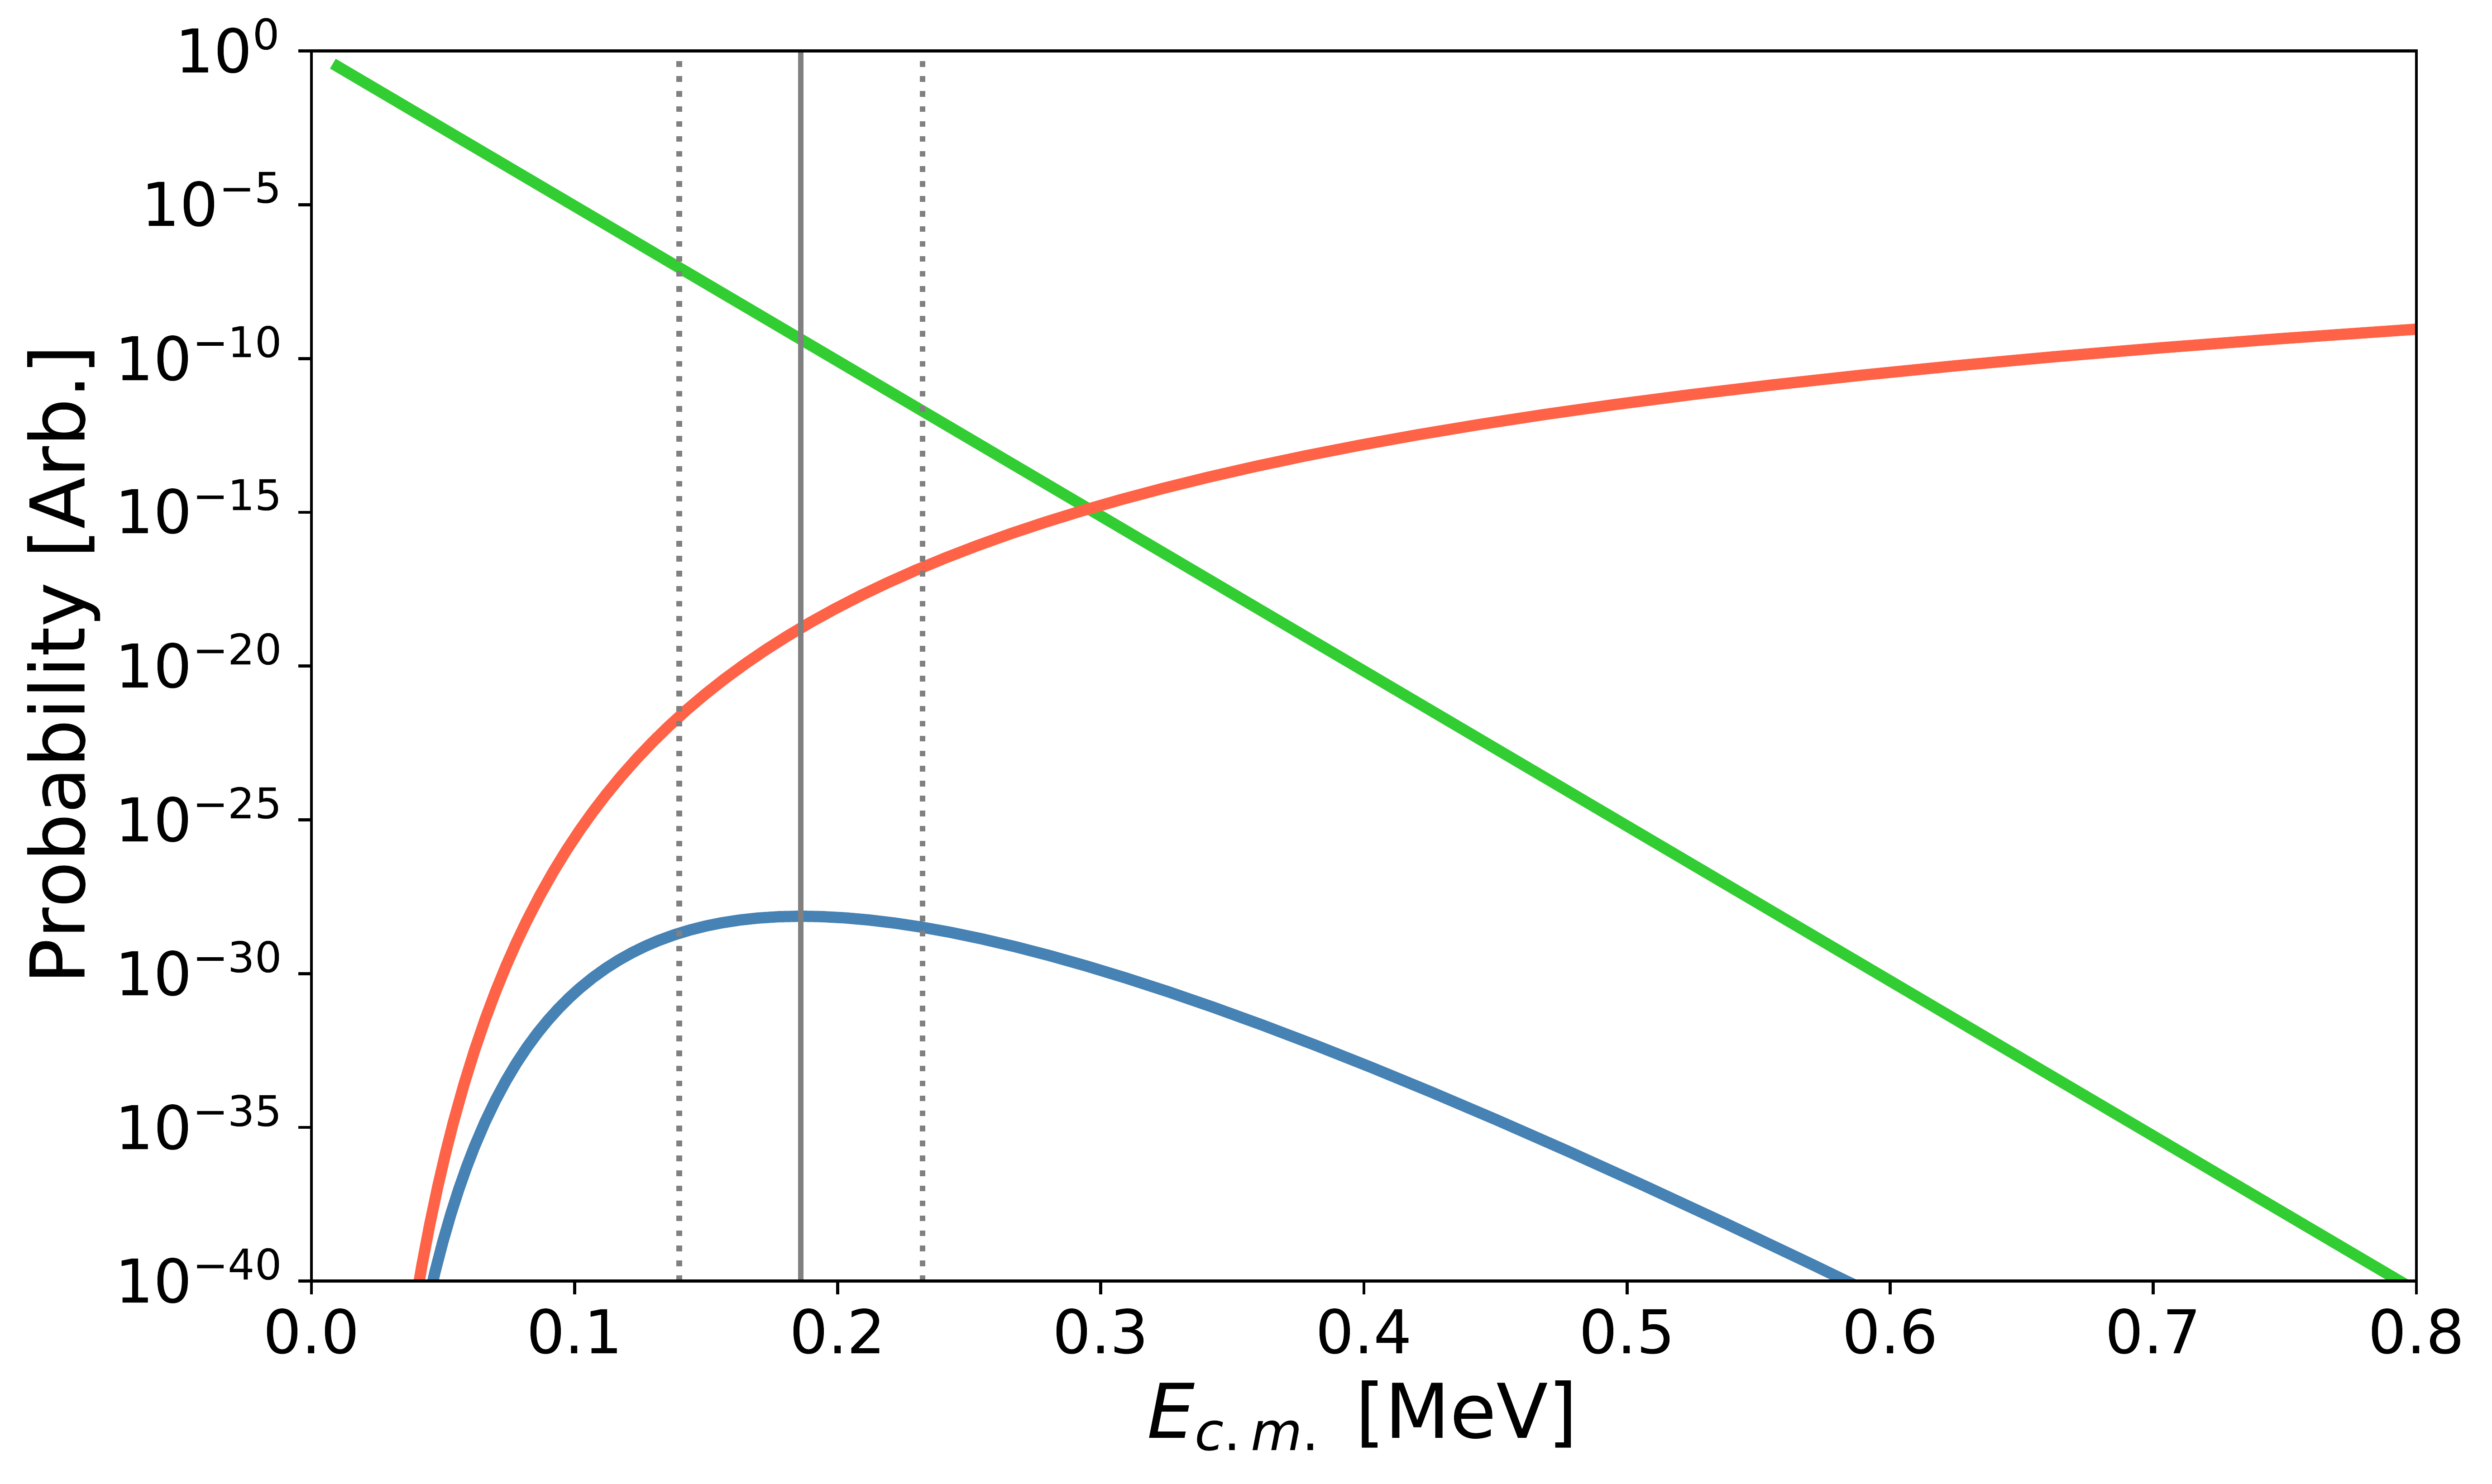
\includegraphics[width=6.5in]{Chapter-2/figs/Gamow_Window.png}};
\node at (5,3.15) {\Huge{$e^{-2\pi\eta}$}};
\node at (5,-0.5) {\Huge{$e^{-E/kT}$}};
\node[rotate=-20] at (1,-1.575) {\Huge{$e^{-2\pi\eta} e^{-E/kT}$}};
\node at (-5,2) {\large{$E_{0} \pm \frac{\Delta}{2}$}};
\draw[line width = 0.1 mm] (-4.9,1) -- (-3,1);
\draw[>=triangle 45, line width = 0.1 mm, ->] (-4.9,1) -- (-4.9,1.7);
\node at (0.5,3.9) (A) {\large{$T = 100$ MK}};
\node[draw=black, fit=(A)] {};
\end{tikzpicture}
\caption{\label{fig:Gamow_Window}The Gamow window, $E_{0} \pm \Delta/2$, for the $^{39}\mathrm{K}(p,\gamma)^{40}\mathrm{Ca}$ reaction at 100 MK. The Gamow factor $e^{-2 \pi \eta}$ is shown in red; the Maxwell-Boltzmann factor $e^{-E/kT}$ is shown in green, and the Gamow peak $e^{-2 \pi \eta} e^{-E/kT}$ is shown in blue. The resonances that contribute significantly to the reaction rate at this temperature will have energies within the Gamow window, between about 140 keV and 230 keV.}
\end{figure}

\subsection{Narrow Resonances} \label{subsec:narrow_resonances}

An isolated resonance at the resonance energy $E_{r}$ is described by the Breit-Wigner cross-section \cite{Breit1936}
\begin{equation} \label{eqn:BW_Cross}
\sigma_{\mathrm{BW}}(E) = \frac{\lambda^{2}}{4 \pi} \, \omega \frac{\Gamma_{a}(E) \, \Gamma_{b}(E)}{\left(E - E_{r}\right)^{2} + \Gamma(E)^{2}/4},
\end{equation}
where $\lambda$ is the deBroglie wavelength, defined by $\lambda^{2}/2 = (\pi \hbar)^{2} / (\mu_{01} E)$; $\Gamma_{a}(E)$ and $\Gamma_{b}(E)$ are the entrance channel and exit channel partial widths, respectively; $\Gamma(E)$ is the total width, and $\omega$ is the spin factor, defined as
\begin{equation}
\omega = \frac{(2J+1)}{(2J_{0}+1) (2J_{1}+1)},
\end{equation}
where $J$ is the resonance spin, and $J_{0}$ and $J_{1}$ are the spins of the interacting particles. Substituting Eqn. \ref{eqn:BW_Cross} into Eqn. \ref{eqn:reaction_rate}, the reaction rate per particle pair arising from an isolated resonance becomes
\begin{equation}
\left\langle \sigma v \right\rangle_{01} = \frac{\sqrt{2 \pi} \hbar^{2}}{\left(\mu_{01} k T\right)^{3/2}} \, \omega \int_{0}^{\infty} \frac{\Gamma_{a}(E) \, \Gamma_{b}(E)}{\left(E - E_{r}\right)^{2} + \Gamma(E)^{2}/4} \, e^{-E/kT} \, dE.
\end{equation}

Consider the partial widths $\Gamma_{i}$ and the Maxwell-Boltzmann factor $e^{-E/kT}$ varying slowly with energy over the width of the resonance. In this situation, the resonance is considered narrow, and these factors can be treated as being independent of energy over this energy range. The reaction rate is then written as
\begin{align}
\left\langle \sigma v \right\rangle_{01} &= \frac{\sqrt{2 \pi} \hbar^{2}}{\left(\mu_{01} k T\right)^{3/2}} \, \omega \Gamma_{a} \, \Gamma_{b} \, e^{-E_{r}/kT} \int_{0}^{\infty} \frac{dE}{\left(E - E_{r}\right)^{2} + \Gamma(E)^{2}/4} \nonumber \\
&= \frac{\sqrt{2 \pi} \hbar^{2}}{\left(\mu_{01} k T\right)^{3/2}} \, \omega \Gamma_{a} \, \Gamma_{b} \, e^{-E_{r}/kT} \, \frac{2}{\Gamma} \, \left. \arctan\left( \frac{E - E_{r}}{\Gamma/2} \right)\right|_{0}^{\infty} \nonumber \\
&= \left(\frac{2 \pi}{\mu_{01} k T}\right)^{3/2} \hbar^{2} \, \omega \frac{\Gamma_{a} \, \Gamma_{b}}{\Gamma} \, e^{-E_{r}/kT},
\end{align}
where the last line results from the further approximation of narrow resonances, $E_{r} >> \Gamma$, which makes the lower bound of integration effectively $-\infty$. The quantity
\begin{equation}
\omega \gamma \equiv \omega \frac{\Gamma_{a} \, \Gamma_{b}}{\Gamma}
\end{equation}
is defined as the \emph{resonance strength} because it is proportial to the maximum cross section multiplied by the total resonance width, $\omega \gamma \propto \sigma_{\mathrm{max}} \Gamma$. The reaction rate per particle pair for multiple isolated, narrow resonances forms an incoherent sum,
\begin{equation}
\left\langle \sigma v \right\rangle_{01} = \left(\frac{2 \pi}{\mu_{01} k T}\right)^{3/2} \hbar^{2} \, \sum_{i} \, (\omega \gamma)_{i} \, e^{-E_{r, \, i}/kT}.
\end{equation}
The calculation of partial widths differs between particles and $\gamma$-rays. The following discussion will consider charged-particles and $\gamma$-rays only. For a discussion of neutron partial widths, see Ref. \cite{Iliadis2015}.

\subsection{Particle Partial Widths}

The charged-particle partial width for channel $c$ is
\begin{equation} \label{eqn:partial_width}
\Gamma_{c}(E) = \frac{2 \hbar^{2}}{\mu_{01} R^{2}} \, P_{c}(E) \, C^{2}S \, \theta_{\mathrm{sp}, \, c},
\end{equation}
where the channel radius $R$ is defined by $R = R_{0} \left( A_{0}^{1/3} + A_{1}^{1/3} \right)$; the penetration factor $P_{c}(E)$ can be calculated as
\begin{equation}
P_{c}(E) = \frac{\rho}{F^{2}(E) + G^{2}(E)},
\end{equation}
where $\rho = 0.21874 \, R \, \sqrt{\mu_{01} E}$ and $F$ and $G$ are the energy dependent Coulomb wave functions; $C^{2}S$ is the spectroscopic factor, sometimes simply referred to as $S$, where $C$ is the isospin Clebsch-Gordon coefficient, and $\theta_{\mathrm{sp}, \, c}$ is the dimensionless single-particle reduced width. The charged-particle partial width can be thought of as being proportional to the probability of the particle being emitted from the compound nucleus. Each of the latter three quantities in Eqn. \ref{eqn:partial_width} contribute to this probability. The penetration factor $P_{c}(E)$ represents the probability of overcoming or tunneling through the Coulomb barrier to reach the nuclear surface. The dimensionless single-particle reduced width $\theta_{\mathrm{sp}, \, c}$ represents the probability that the particle occupies the exact single-particle shell-model state of the resonance at the nuclear surface. Finally, the spectroscopic factor $C^{2}S$ is a measure of how much the populated state resembles that single-particle shell-model state. Although $C^{2}S$ is model-dependent, it is the only quantity in Eqn. \ref{eqn:partial_width} that is based on measurement, as will be clear in Section \ref{subsec:DWBA}.

The dimensionless single-particle reduced width is given by
\begin{equation}
\theta_{\mathrm{sp}, \, c} = \frac{R}{2} | u_{\mathrm{sp}, \, c}(R) |^{2},
\end{equation}
where $u_{\mathrm{sp}, \, c}(R)$ is the single-particle radial wavefunction evaluated at the channel radius, which is normalized to unity as in
\begin{equation}
\int_{0}^{R} |u_{\mathrm{sp}, \, c}(R)|^{2} \, r^{2} \, dr = 1.
\end{equation}
One method of numerically calculating $\theta_{\mathrm{sp}, \, c}$ is to vary the parameters of the single-particle potential until a resonance is produced at the binding energy. This is performed, for example, by the code \texttt{BIND}, detailed in Ref. \cite{Iliadis1997}. Another procedure, performed for $^{39}\mathrm{K}(p, \gamma)^{40}\mathrm{Ca}$ in Sec. \ref{subsec:partial_widths}, is to use the weak binding approximation. This approximation is required if the nuclear reaction code used in the determination of $C^{2}S$ only handles bound states, as is the case with \texttt{Fresco} \cite{Thompson1988,Fresco}. This method assumes unbound states are weakly bound (by $\lesssim 50$ keV), and therefore $u_{\mathrm{sp}, \, c}(R)$ is the bound state radial wavefuction evaluated at the channel radius. The channel radius $R$ is selected to represent the nuclear surface, where the wavefunctions for the bound state and unbound state are equivalent.

A fact that appears troubling for the weak binding approximation at first glance is that both $C^{2}S$ and $\theta_{\mathrm{sp}, \, c}$ depend linearly on the binding energy, assuming $R$ is chosen at the nuclear surface. Therefore, both quantities will diverge from unbound calculations at high binding energies. However, as Ref. \cite{Harrouz2023} has shown for the proton-transfer reaction $^{30}\mathrm{Si}(^{3}\mathrm{He},d)^{31}\mathrm{P}$, $C^{2}S$ decreases as a function of binding energy at roughly the same rate as $\theta_{\mathrm{sp}, \, c}$ increases, such that their product is balanced. The only signficant energy dependence from Eqn. \ref{eqn:partial_width} therefore comes from the penetration factor $P_{c}(E)$, which can easily be evaluated for unbound energies without the use of the weak binding approximation.

\subsection{$\gamma$-ray Partial Widths}
The $\gamma$-ray partial width for a single transition is
\begin{equation}
\Gamma_{\gamma}(\bar{\omega}, E_{\gamma}) = \frac{8 \pi (L + 1)}{L\left[(2L + 1)!!\right]^{2}} \left(\frac{E_{\gamma}}{\hbar c}\right)^{2L+1} B(\bar{\omega}L),
\end{equation}
where $\bar{\omega}$ represents either electric or magnetic radiation; $E_{\gamma}$ is the $\gamma$-ray transition energy; $L$ is the $\gamma$-ray multipolarity, and $B$ is the branching ratio. The $\gamma$-ray partial width at the incoming particle energy $E$ can be scaled with respect to that of the resonance energy $E_{r}$ as in
\begin{equation}
\Gamma_{\gamma}(E) = \Gamma_{\gamma}(E_{r}) \left(\frac{E + Q - E_{f}}{E_{r} + Q - E_{f}}\right)^{2L+1},
\end{equation}
where $Q$ is the $Q$-value, or equivalently, the particle separation energy, and $E_{f}$ is the final excitation energy of the $\gamma$-decay.

%%%%%%%%%%%%%%%%%%%%%%%%%%%%%%%%%%%%%%%%%%%%%%%%%%%%%%%%%%%%%%%%%%%%%%%%%%%%%%%%%%%%%%%%%%%%%
\section{Transfer Reactions}

% This will be the last section of this chapter
% Theory leading to C2S definition from overlap functions

% Random Ch 6 note when I was going to discuss transfer reactions there:
%Chapter \ref{chap:reactions} described the proton-capture reaction rate as a function of experimental quantities, such as the proton partial-width $\Gamma_{p}$ and the $\gamma$-ray partial width $\Gamma_{\gamma}$. This section will describe how the proton partial-width



\subsection{Optical Model} \label{subsec:Optical_Model}

\subsection{Distorted Wave Born Approximation} \label{subsec:DWBA}

% Theoretical model, similar to Caleb's Section in his Chapter 2

% For a surface level explanation (good for defense questions! and for intro to section), see Krane pg. 421-424.

% Include Zero-range approximation

%\subsection{Spectroscopic Factors} \label{subsec:C2S}
% Might not need this section (should be covered in both Narrow Resonance and DWBA sections)
%\subsection{Proton Partial Widths} \label{subsec:PartialWidths}
% Might not need this section (should be covered in Narrow Resonance section)